\documentclass{beamer}
\usetheme{Madrid}

\usepackage{amsmath, amssymb}
\usepackage{listings}
\usepackage{xcolor}
\lstset{
	    language=Python,
	        basicstyle=\ttfamily\small,
		    keywordstyle=\color{blue},
		        commentstyle=\color{green!60!black},
			    stringstyle=\color{red},
			        breaklines=true,
				    frame=single
			    }
			    
\title[PD Controller Design]{Control Systems Problem}
\author{Darsh Pankaj Gajare --- EE25BTECH11020}
\date{}

\begin{document}

%----------- Title Page -----------
\begin{frame}
  \titlepage
\end{frame}

%----------- Problem Statement -----------
\begin{frame}{Question}
A control system with a PD controller is shown. If the velocity error constant $K_v = 1000$ and the damping ratio $\zeta = 0.5$, then the values of $K_P$ and $K_D$ are:
	\begin{figure}
		\centering
		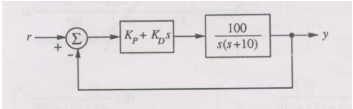
\includegraphics[scale=0.5]{figs/question.png}
	\end{figure}
	\begin{enumerate}
		\item $K_P=100$, $K_D=0.09$
		\item $K_P=100$, $K_D=0.9$
		\item $K_P=10$, $K_D=0.09$
		\item $K_P=10$, $K_D=0.9$
	\end{enumerate}
\end{frame}

%----------------------------------------
\begin{frame}{Given}

\begin{itemize}
\item Controller: $K_p + K_D s$
\item Plant: $\dfrac{100}{s(s+10)}$
\item Unity feedback system
\item $K_v = 1000$
\item $\zeta = 0.5$
\end{itemize}

Find:
\[
K_p, \quad K_D
\]

\end{frame}

%----------------------------------------
\begin{frame}{Step 1: Open-loop Transfer Function}

\[
G(s) = \frac{100(K_p + K_D s)}{s(s+10)}
\]

\end{frame}

%----------------------------------------
\begin{frame}{Step 2: Velocity Error Constant}

\[
K_v = \lim_{s \to 0} sG(s)
\]

\[
K_v = \lim_{s \to 0} \frac{100(K_p + K_D s)}{s+10}
\]

As $s \to 0$:
\[
K_v = \frac{100K_p}{10} = 10K_p
\]

\[
10K_p = 1000 \Rightarrow K_p = 100
\]

\end{frame}

%----------------------------------------
\begin{frame}{Step 3: Characteristic Equation}

\[
1 + G(s) = 0
\]

\[
s(s+10) + 100(K_p + K_D s) = 0
\]

\[
s^2 + (10 + 100K_D)s + 100K_p = 0
\]

\end{frame}

%----------------------------------------
\begin{frame}{Step 4: Standard Form Comparison}

\[
s^2 + 2\zeta \omega_n s + \omega_n^2 = 0
\]

Matching terms:
\[
\omega_n^2 = 100K_p
\]
\[
2\zeta \omega_n = 10 + 100K_D
\]

\end{frame}

%----------------------------------------
\begin{frame}{Step 5: Natural Frequency}

\[
\omega_n^2 = 100 \times 100 = 10000
\]

\[
\omega_n = 100
\]

\end{frame}

%----------------------------------------
\begin{frame}{Step 6: Damping Ratio}

\[
2\zeta \omega_n = 2 \times 0.5 \times 100 = 100
\]

\[
10 + 100K_D = 100
\]

\[
100K_D = 90 \Rightarrow K_D = 0.9
\]

\end{frame}

%----------------------------------------
\begin{frame}{Final Answer}

\begin{alertblock}{Result}
\[
K_p = 100,\quad K_D = 0.9
\]
\end{alertblock}

\end{frame}

	\lstinputlisting{codes/verify.py}

%--------------------------------

\begin{frame}{Velocity Error Constant ($K_v$)}

\begin{block}{Definition}
\[
K_v = \lim_{s \to 0} sG(s)
\]
\end{block}

\begin{block}{Meaning}
$K_v$ measures how well a system tracks a \textbf{ramp input} (continuously increasing input).
\end{block}

\begin{block}{Steady-State Error}
\[
e_{ss} = \frac{1}{K_v}
\]
\end{block}

\begin{block}{Practical Interpretation}
\begin{itemize}
\item Higher $K_v$ $\Rightarrow$ smaller tracking error
\item Lower $K_v$ $\Rightarrow$ larger tracking error
\end{itemize}
\end{block}

\begin{block}{Example}
For $K_v = 1000$:
\[
e_{ss} = \frac{1}{1000} = 0.001
\]
$\Rightarrow$ Excellent tracking performance
\end{block}

\end{frame}
\begin{frame}{Velocity Error Constant ($K_v$)}


\begin{block}{Example}
Cruise control:
\begin{itemize}
\item High $K_v$ $\Rightarrow$ car follows increasing speed closely
\item Low $K_v$ $\Rightarrow$ car falls behind desired speed
\end{itemize}
\end{block}

\end{frame}
%--------------------------------
\begin{frame}{Ramp Tracking Demonstration}

\begin{figure}
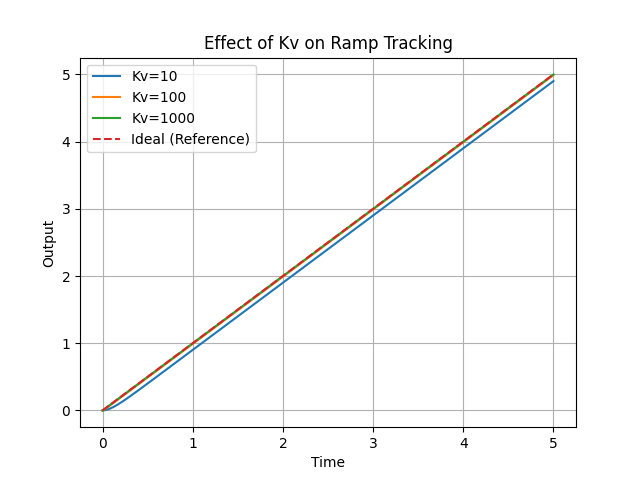
\includegraphics[width=0.9\linewidth]{figs/Kv.png}
\caption{Higher $K_v$ improves tracking of ramp input}
\end{figure}

\end{frame}

%--------------------------------
\begin{frame}{Damping Ratio ($\zeta$)}

\begin{block}{Definition}
\[
\zeta = \text{Damping Ratio}
\]
\end{block}

\begin{block}{Standard Form}
\[
s^2 + 2\zeta \omega_n s + \omega_n^2 = 0
\]
\end{block}

\begin{block}{Meaning}
$\zeta$ determines how \textbf{smooth or oscillatory} the system response is.
\end{block}

\begin{block}{Behavior}
\begin{itemize}
\item $0 < \zeta < 1$ $\Rightarrow$ Oscillatory (underdamped)
\item $\zeta = 0.5$ $\Rightarrow$ Moderate overshoot
\item $\zeta = 1$ $\Rightarrow$ No oscillation (critical damping)
\item $\zeta > 1$ $\Rightarrow$ Slow response (overdamped)
\end{itemize}
\end{block}



\end{frame}
\begin{frame}{Damping Ratio ($\zeta$)}



\begin{block}{Practical Meaning}
$\zeta$ determines how \textbf{smoothly the system reaches its target}.
\end{block}



\begin{block}{Example}
Car suspension:
\begin{itemize}
\item Low $\zeta$ $\Rightarrow$ bouncing
\item Proper $\zeta$ $\Rightarrow$ smooth settling
\end{itemize}
\end{block}

\end{frame}
%--------------------------------
\begin{frame}{Damping Demonstration}

\begin{figure}
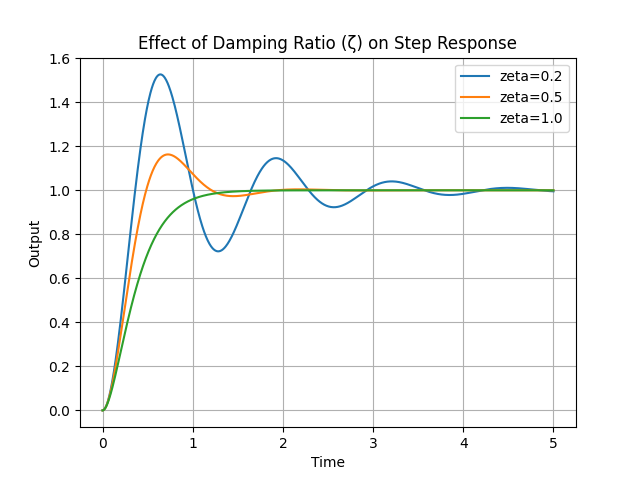
\includegraphics[width=0.9\linewidth]{figs/zeta.png}
\caption{Effect of damping ratio on step response}
\end{figure}

\end{frame}

%--------------------------------
\begin{frame}{Bode Plots of Transfer Function}
\begin{figure}
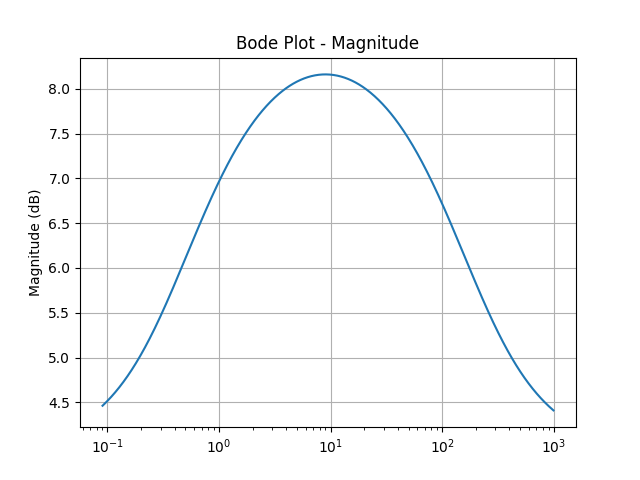
\includegraphics[width=0.9\linewidth]{figs/bodem.png}
\end{figure}
\end{frame}
\begin{frame}
\begin{figure}
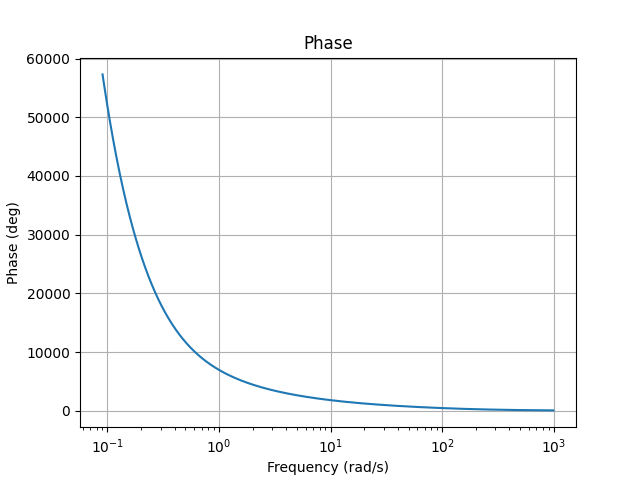
\includegraphics[width=0.9\linewidth]{figs/bodef.png}
\end{figure}
\end{frame}
\end{document}
